%----------------------Нүүр хуудастай хамаатай зүйлс----------------------------
\pagenumbering{roman}
\makefrontpage
\maketitle

\doublespace

% Decleration
\begin{huge}
\textbf{Зохиогчийн баталгаа}
\end{huge} \\ \ \\
\doublespace
Миний бие \@author \ "\@title" \ сэдэвтэй судалгааны ажлыг гүйцэтгэсэн болохыг зарлаж дараах зүйлсийг баталж байна:
\begin{itemize}
\item Ажил нь бүхэлдээ эсвэл ихэнхдээ Монгол Улсын Их Сургуулийн зэрэг горилохоор дэвшүүлсэн болно.
\item Бусдын хийсэн ажлаас хуулбарлаагүй, ашигласан бол ишлэл, зүүлт хийсэн.
\item Ажлыг би өөрөө (хамтарч) хийсэн ба миний хийсэн ажил, үзүүлсэн дэмжлэгийг тайлангийн ажилд тодорхой тусгасан.
\item Ажилд тусалсан бүх эх сурвалжид талархаж байна.
\end{itemize}
\

Гарын үсэг: \underline{\hspace{5cm}}

Огноо: 	\ \ \underline{\hspace{3cm}}

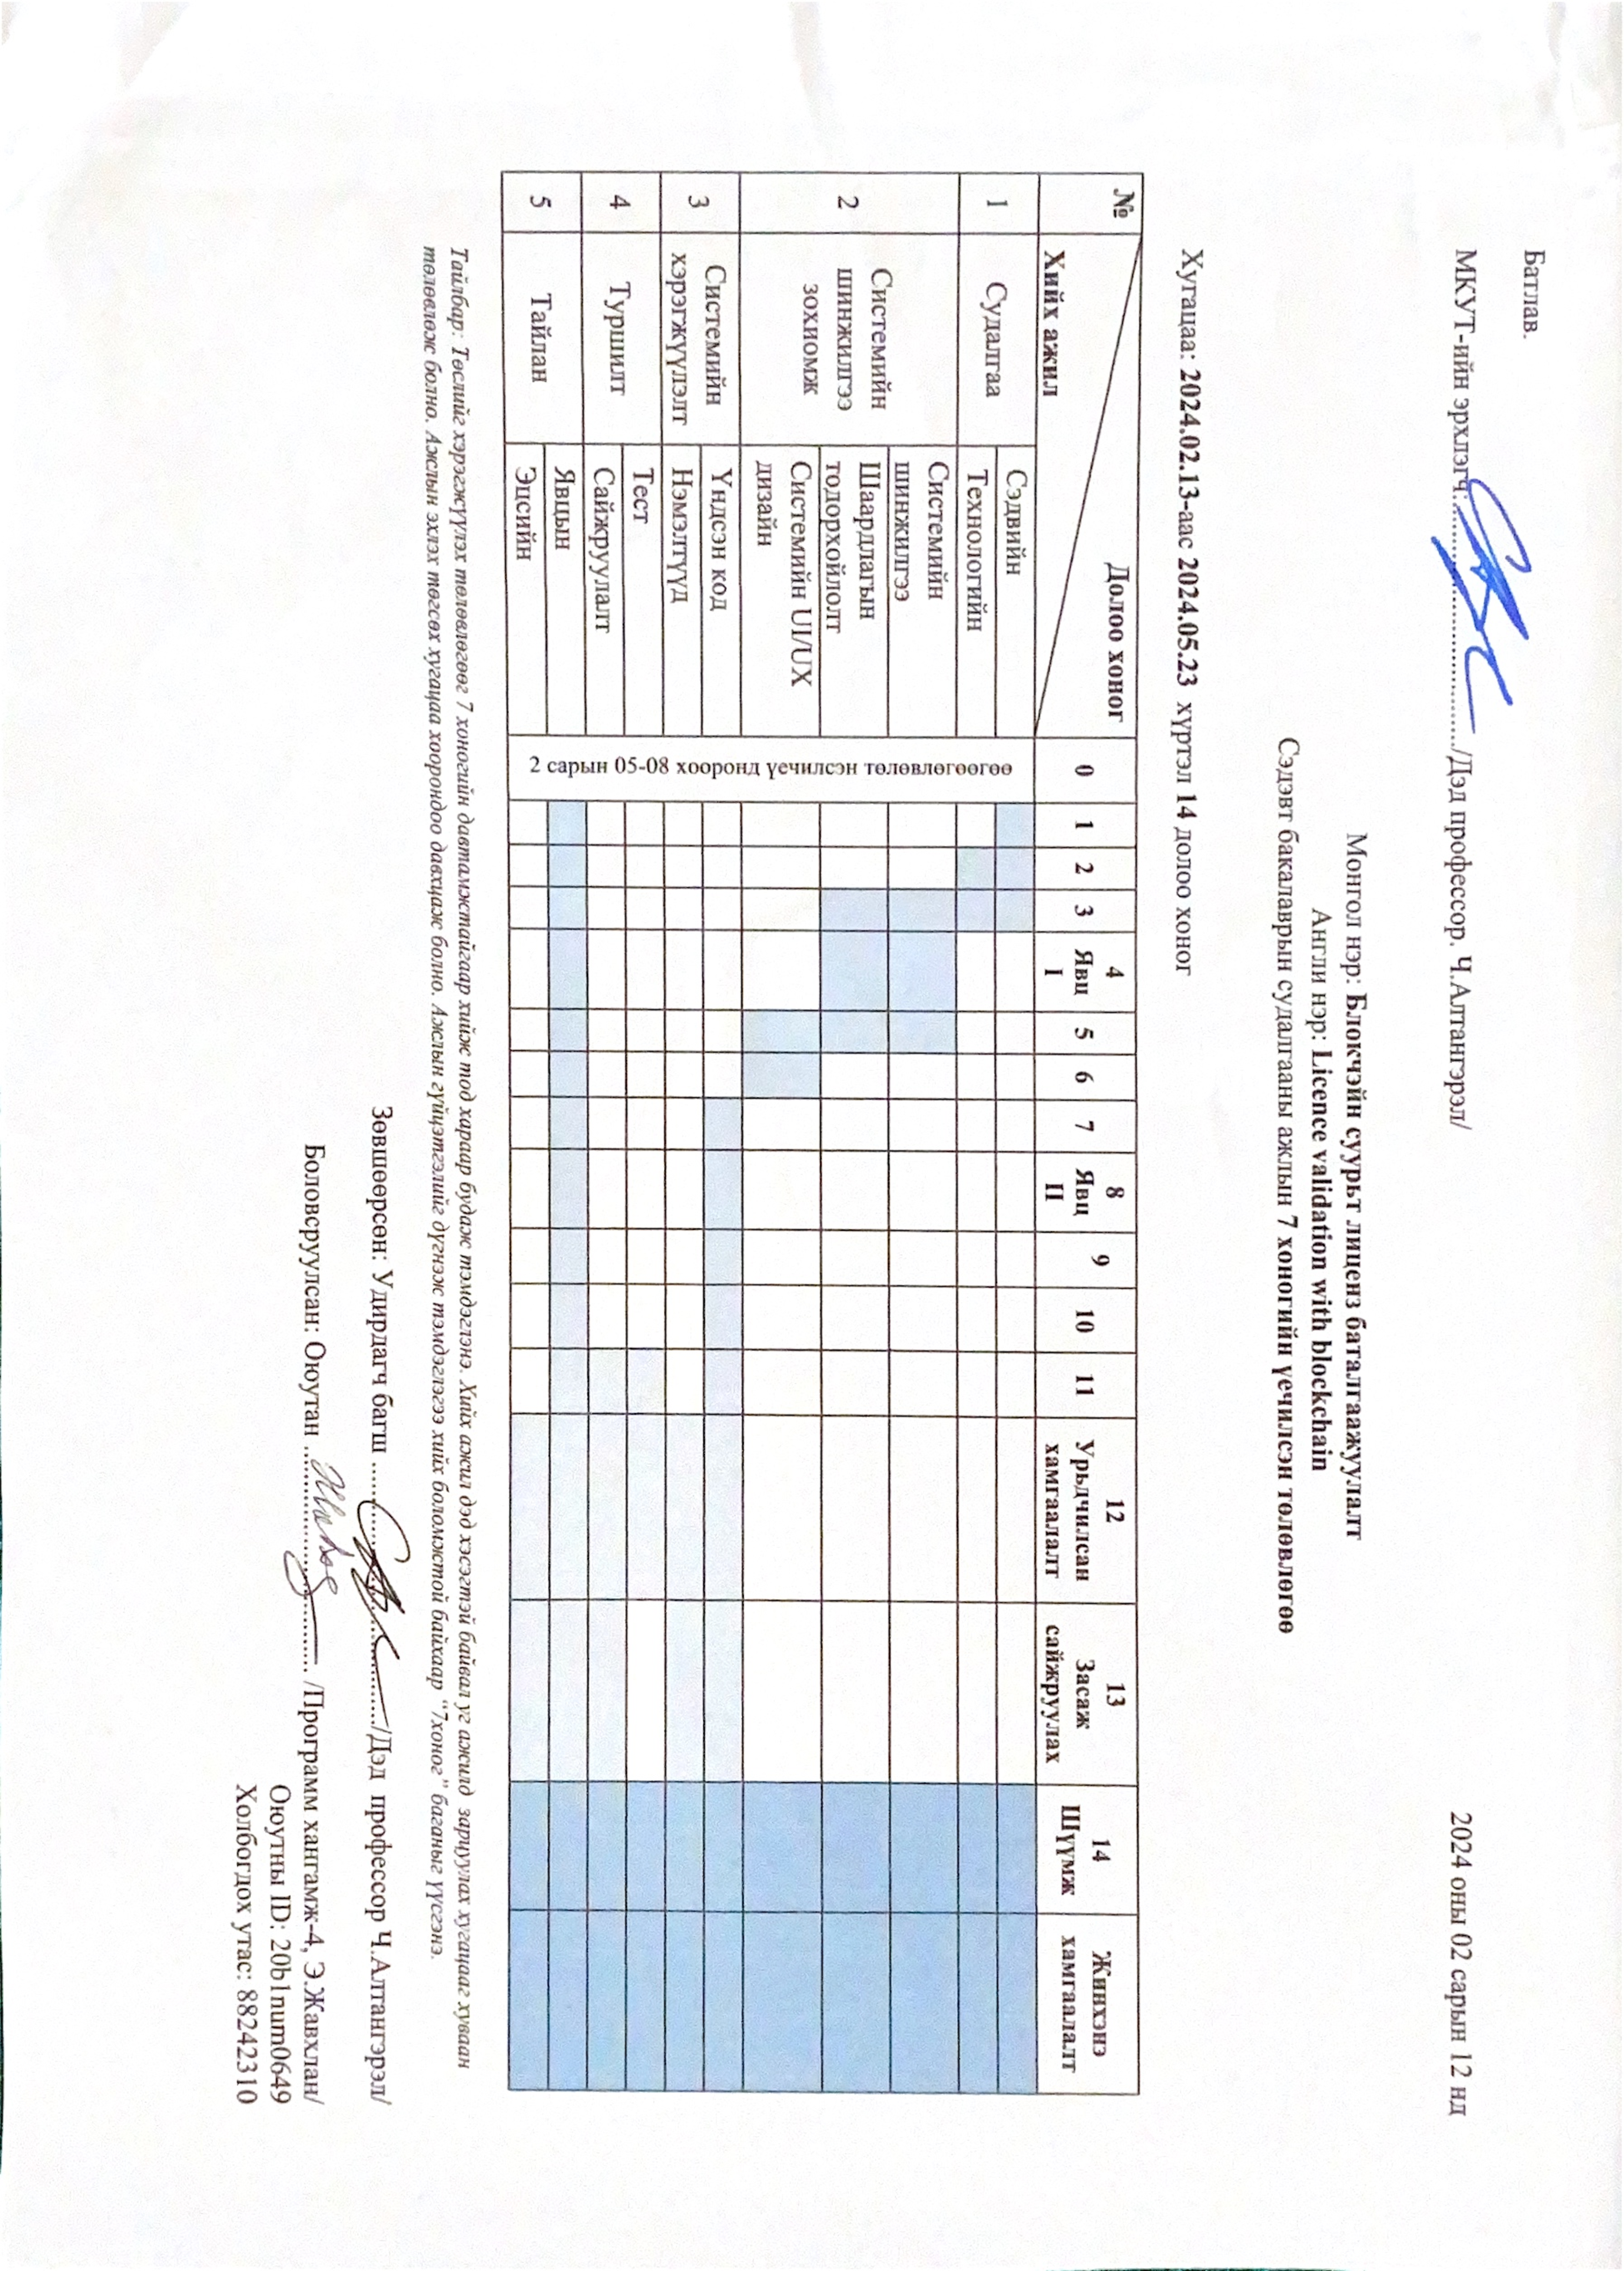
\includepdf[pages=1]{./src/periodic-table.pdf}

\includepdf[pages=1]{./src/todorh.pdf}
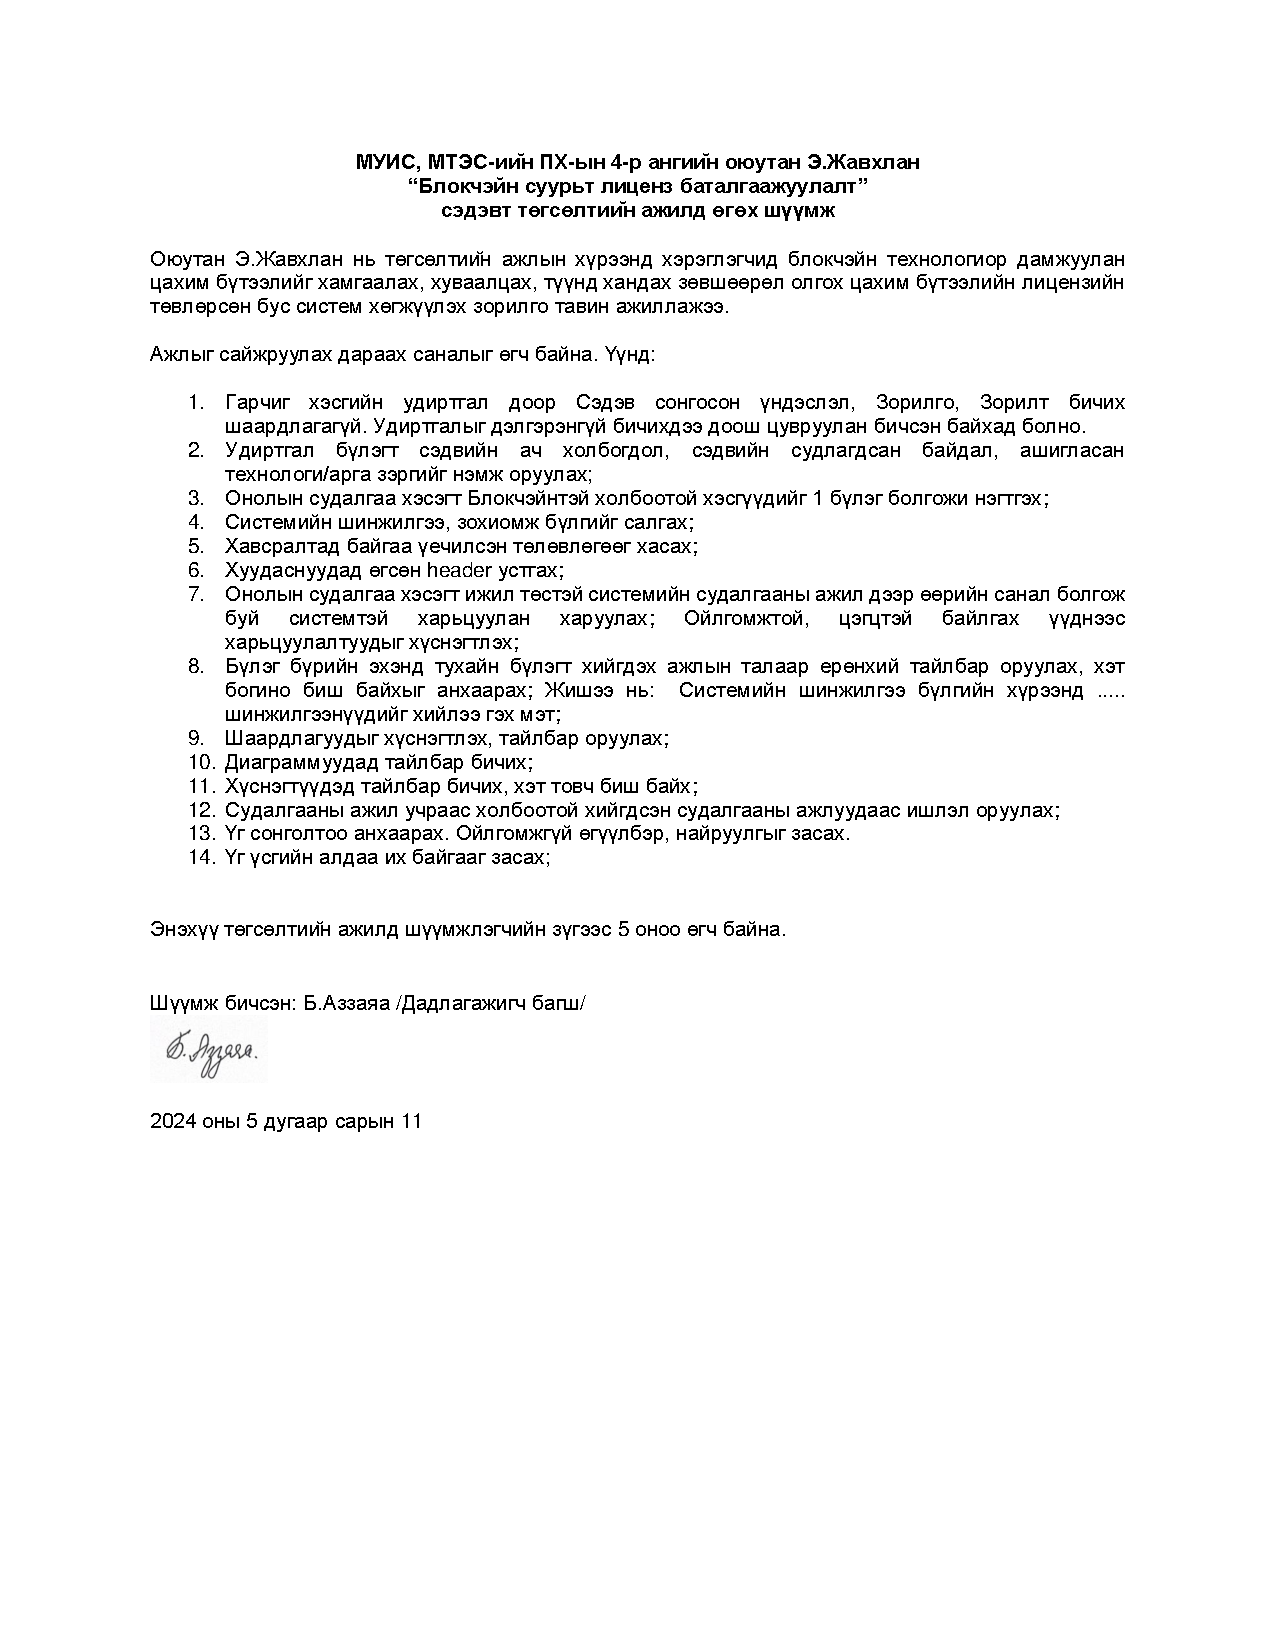
\includepdf[pages=1]{./src/review.pdf}
% Гарчгийг автоматаар оруулна
\setcounter{tocdepth}{1}
\tableofcontents

% Зургийн жагсаалтыг автоматаар оруулна
\listoffigures

% Хүснэгтийн жагсаалтыг автоматаар оруулна
\listoftables

% Кодын жагсаалтыг автоматаар оруулна
\lstlistoflistings

% This puts the word "Page" right justified above everything else.
\newpage
%% \addtocontents{lof}{Зураг~\hfill Хуудас \par}
\newpage
%% \addtocontents{lot}{Хүснэгт~\hfill Хуудас \par}

\renewcommand{\cftlabel}{Зураг}


\doublespace
\pagenumbering{arabic}
